Die Quanten Fourier-Transformation (QFT), transformiert einen Basiszustand $|x\rangle$ zu einem Fourierzustand $|\tilde{x}\rangle$ \cite{Qiskit-Textbook}. Die QFT ist die Anwendung der Diskreten Fourier-Transformation (DFT) auf Quantenzust\"ande, somit unterscheidet diese sich minimal zur Berechnung von Fourierkoeffizienten mittels DFT.
\begin{equation}
  \begin{aligned}
    DFT &\Rightarrow X[k] = \frac{1}{\sqrt{N}}\sum\limits_{j=0}^{N-1}e^{i\frac{2\pi}{N}kj}\cdot x[j] \\[1em]
    QFT &\Rightarrow |\tilde{x}\rangle = \frac{1}{\sqrt{N}}\sum\limits_{j=0}^{N-1}e^{i\frac{2\pi}{N}xj}\cdot|j\rangle
  \end{aligned}
\end{equation}
Die Berechnung der QFT kann somit auf ein Quantenregister \ref{sec:multiple-qubits} ausgef\"uhrt werden. Bei der Quantum Fourier-Transformation entspricht $N = 2^n$, dabei ist $n$ die Anzahl der genutzten Qubits. In \cite{Qiskit-Textbook} wird gezeigt, wie es m\"oglich ist die QFT als Produkt auszuschreiben.
\begin{equation}
  |\tilde{x}\rangle = \frac{1}{\sqrt{N}} \left(|0\rangle + e^{i\frac{2\pi x}{2^1}}|1\rangle\right)\otimes\left(|0\rangle + e^{i\frac{2\pi x}{2^2}}|1\rangle\right)\otimes\dots\otimes\left(|0\rangle + e^{i\frac{2\pi x}{2^n}}|1\rangle\right)
\end{equation}
Aus diesem Produkt l\"asst sich die Schaltung der QFT etwas verst\"andlicher nachvollziehen, denn es werden zur Erstellung der Schaltung pro Qubit ein Hadamard-Gatter und mehrere kontrollierte $R_k$-Gatter ben\"otigt (Abbildung \ref{fig:QFT-Circuit}). Dabei sind $R_k$-Gatter spezifizierte Phasen-Gatter \ref{eq:Rn-Gate}. Die aufgetragene QFT-Schaltung kann
\begin{equation}
\label{eq:Rn-Gate}
P\left(\phi = \frac{2\pi}{2^k}\right) = R_k = \begin{bmatrix}
    1 & 0 \\
    0 & e^{i\frac{2\pi}{2^k}}
    \end{bmatrix}
\end{equation}
\begin{figure}[h]
\centering
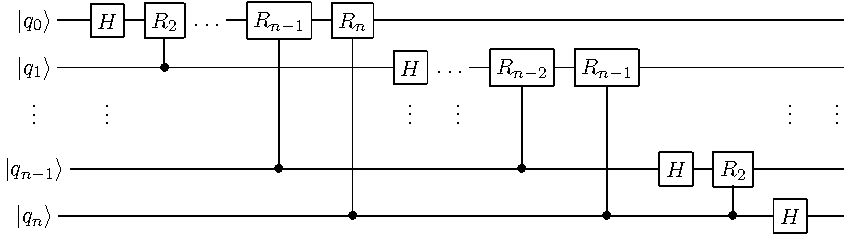
\includegraphics[width=1\textwidth]{figures/QFT.pdf}
\caption{Schaltung der Quantum Fourier-Tranformation (vgl. \cite{nielsen_chuang_2010})}
\label{fig:QFT-Circuit}
\end{figure}
auch invertiert realisiert werden (erstes H-Gatter auf Qubit $|q_n\rangle$). Bei dieser Struktur ist jedoch zu beachten, dass die Ausgabe der Qubits ebenso durch $SWAP$-Gattern umgekehrt werden muss.
In Anhang \ref{chap:anhang} Listing \ref{list:qft} ist die Implementierung der QFT-Schaltung in Qiskit f\"ur $n=3$ Qubits dargestellt. Abbildung \ref{fig:QFT-Bloch} zeigt die Rotation der jeweiligen Zustandvektoren auf der Bloch-Kugel f\"ur das Quantenregister $|5\rangle$, vor und nach Anwendung der Quantum Fourier-Transformation.
\begin{equation}
|101\rangle \xrightarrow{QFT} |\tilde{101}\rangle
\end{equation}

\begin{figure}[h]
\centering
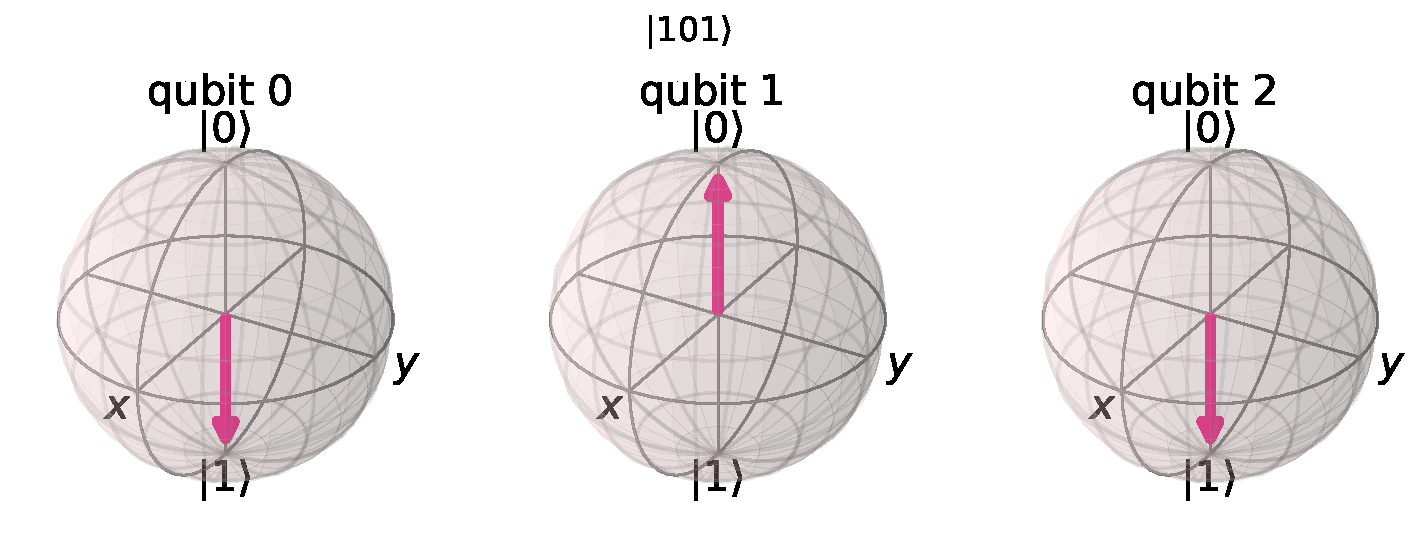
\includegraphics[width=0.9\textwidth]{figures/qft_init.pdf}
\bigbreak
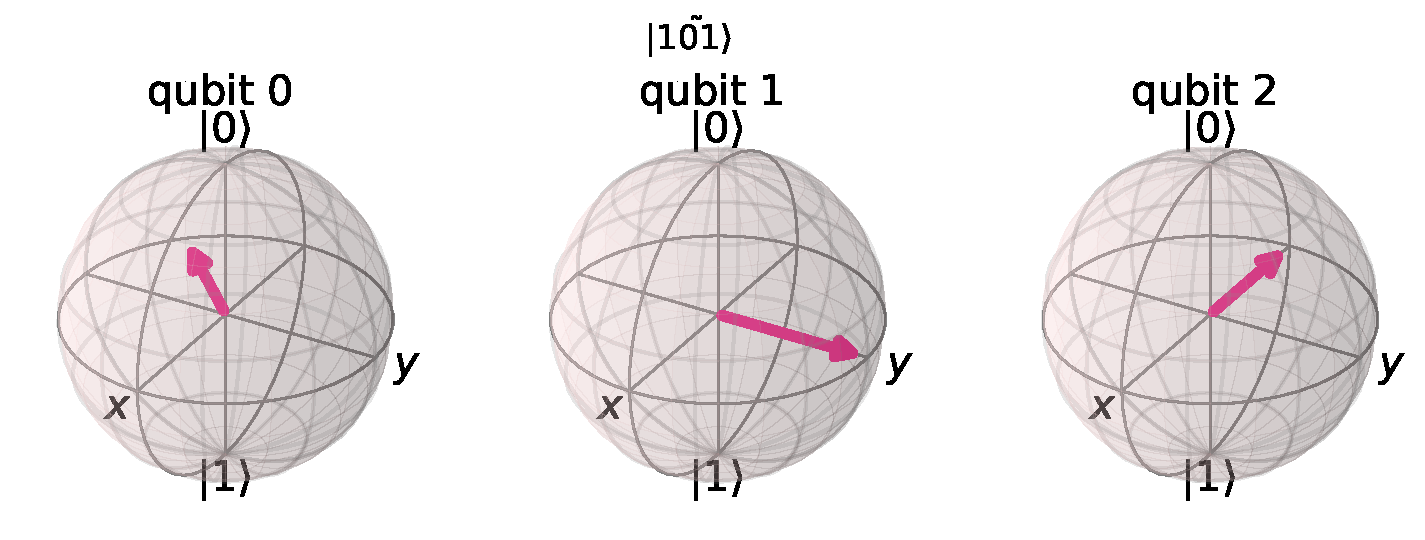
\includegraphics[width=0.9\textwidth]{figures/qft_applied.pdf}
\caption{Rotation auf der Bloch-Kugel durch Anwenden der QFT (vgl. \cite{Qiskit-Textbook})}
\label{fig:QFT-Bloch}
\end{figure}
